\documentclass[dcc,uchile,sol]{fcfmcourse}
\usepackage{teoria}
\usepackage[utf8x]{inputenc}
\usepackage{amsmath}
\usepackage{amsfonts,setspace}
\usepackage{listings}
\usepackage{hyperref}
\usepackage{color}
\usepackage{tikz}





\definecolor{pblue}{rgb}{0.13,0.13,1}
\definecolor{pgreen}{rgb}{0,0.5,0}
\definecolor{porange}{rgb}{0.9,0.5,0}
\definecolor{pgrey}{rgb}{0.46,0.45,0.48}

\lstset{language=Java,
  showspaces=false,
  showtabs=false,
  breaklines=true,
  showstringspaces=false,
  breakatwhitespace=true,
  commentstyle=\color{porange},
  keywordstyle=\color{pblue},
  stringstyle=\color{pgreen},
  basicstyle=\ttfamily,
  moredelim=[il][\textcolor{pgrey}]{$ $},
  moredelim=[is][\textcolor{pgrey}]{\%\%}{\%\%}
}

\newenvironment{codebox} {\small \ttfamily \obeylines \begingroup \setstretch{-2.4}} {\endgroup}

% COmpletar titulo
\title{Auxiliar 2 - Invariantes y Diagramas de Estado}
\course[CC3001]{Algoritmos y Estructuras de Datos}
\professor{Nelson Baloian}
\professor{Patricio Poblete}
\assistant{Gabriel Azócar, Manuel Cáceres}
\assistant{Michel Llorens, Sergio Peñafiel}


\begin{document}
\maketitle

\vspace{-1ex}


\begin{problems}
\problem \underline{\textbf{Misterio}}\\
Considere el siguiente extracto de código Java:
\begin{lstlisting}[language=Java, frame=single]
...
int f = 0;
int g = 1;
for (int i = 1; i <= N; i++) {
    f = f + g;
    g = f - g;
}
System.out.println(f);
...
\end{lstlisting}

\begin{enumerate}[a)]
    \item Complete el código para hacerlo funcional, compile y ejecútelo. ¿Qué hace?
    \item Deduzca el invariante utilizado en el código.
    \item Programe lo mismo de manera recursiva ¿Qué diferencias hay entre estas dos implementaciones? % Aca también se puede hablar de recursion mal hecha
    \item Programe lo mismo de manera iterativa utilizando otro invariante.
\end{enumerate}

%%Implementar alguno de los algoritmos de ordenación cuadráticos vistos en clases
\problem \underline{\textbf{InsertionSort}}\\
El algoritmo de ordenación por inserción o ``InsertionSort'', posee el siguiente invariante:
\begin{itemize}
    \item $a[i] < a[i+1], \forall i \in \{0,\ldots, k-2\}$
\end{itemize}
Luego rompe el invariante considerando el siguiente elemento en el arreglo ($a[k]$) y lo ``inserta'' (haciendo intercambios de elementos consecutivos) en su posición correspondiente.
\begin{enumerate}[a)]
    \item Ordene (ascendentemente) con ``InsertionSort'' el siguiente arreglo [5, 4, 3, 2, 1] ¿Cuántas comparaciones se realizaron en el proceso?
    \item Ahora ordene [1, 2, 3, 4, 5] y cuente el número de comparaciones
    \item Implemente ``InsertionSort'' en Java usando el invariante correspondiente, para esto escriba la función \texttt{static void insertionSort(int[] a)}
\end{enumerate}
\newpage
\problem \underline{\textbf{Secuencias}}
\begin{enumerate}[a)]
    \item Usando invariante cree la función \texttt{static double f(int N)} que calcula la función matemática:
    \begin{equation*}
        f(n) = 1 + \frac{1}{2} + \frac{1}{3} + \ldots + \frac{1}{N}
    \end{equation*}
    \item Usando un diagrama de estados cree la función \texttt{static double g(int N)} que calcula la función matemática:
    \begin{equation*}
        g(n) = 1 - \frac{1}{2} + \frac{1}{3} - \ldots \pm \frac{1}{N}
        % El final podría ser (-1)^(N+1) para que quede más claro
    \end{equation*}
\end{enumerate}

%%Problema de diagramas de estado un poco mas avanzado
\problem \underline{\textbf{Desechos máquina}}

Para la elaboración de cierto producto se tiene una máquina que necesita 2 recursos A y B los cuales los recibe por conductos separados, estos se cargan en compartimientos y cuando se tienen ambos se puede formar el producto final.

En un instante de tiempo la máquina recibe uno de los dos recursos con igual probabilidad. Al recibir un recurso, si la máquina no contaba con este entonces lo carga. Si ya tenia un recurso de este tipo entonces es desechado para no generar sobrecarga. Al tener ambos inmediatamente se crea un producto y ambos compartimientos quedan vacíos.

Un ingeniero establece que la producción es rentable si se desecha a lo más un 35\% del material. ¿Cree que la máquina sería rentable?

\begin{enumerate}
    \item Cree la función \texttt{static char recibeRecurso()} que devuelve con igual probabilidad los caracteres \texttt{A} o \texttt{B}.
    \item Cree un diagrama de estados para el funcionamiento de la máquina.
    
    \begin{solution}
   \begin{center}
    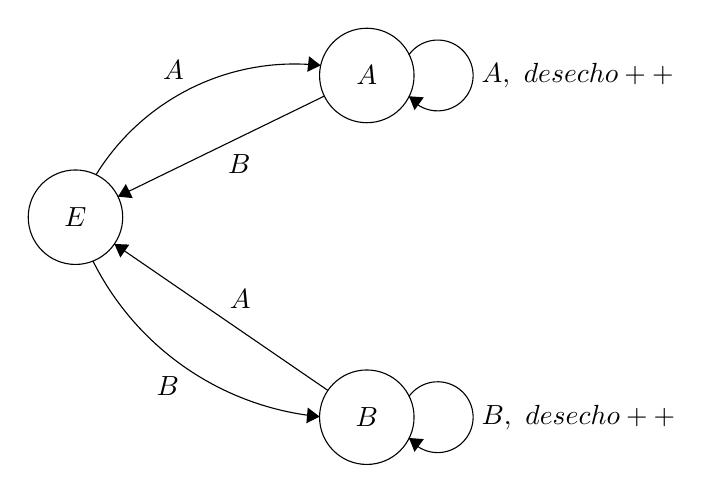
\begin{tikzpicture}[scale=0.2]
   \tikzstyle{every node}+=[inner sep=0pt]
    \draw [black] (20.4,-24.1) circle (3);
    \draw (20.4,-24.1) node {$E$};
    \draw [black] (38.9,-15.1) circle (3);
   \draw (38.9,-15.1) node {$A$};
    \draw [black] (38.9,-36.8) circle (3);
    \draw (38.9,-36.8) node {$B$};
    \draw [black] (35.904,-36.764) arc (-95.46926:-153.46888:18.005);
    \fill [black] (35.9,-36.76) -- (35.15,-36.19) -- (35.06,-37.19);
    \draw (26.26,-34.18) node [below] {$B$};
    \draw [black] (41.58,-35.477) arc (144:-144:2.25);
    \draw (46.15,-36.8) node [right] {$B,\mbox{ }desecho++$};
    \fill [black] (41.58,-38.12) -- (41.93,-39) -- (42.52,-38.19);
    \draw [black] (36.43,-35.1) -- (22.87,-25.8);
   \fill [black] (22.87,-25.8) -- (23.25,-26.66) -- (23.82,-25.84);
    \draw (30.87,-29.95) node [above] {$A$};
    \draw [black] (21.706,-21.405) arc (148.33883:83.54576:14.807);
    \fill [black] (35.97,-14.46) -- (35.23,-13.88) -- (35.12,-14.87);
    \draw (26.62,-15.36) node [above] {$A$};
    \draw [black] (36.2,-16.41) -- (23.1,-22.79);
    \fill [black] (23.1,-22.79) -- (24.04,-22.89) -- (23.6,-21.99);
    \draw (30.8,-20.11) node [below] {$B$};
    \draw [black] (41.58,-13.777) arc (144:-144:2.25);
    \draw (46.15,-15.1) node [right] {$A,\mbox{ }desecho++$};
    \fill [black] (41.58,-16.42) -- (41.93,-17.3) -- (42.52,-16.49);
    \end{tikzpicture}
   \end{center}
  \end{solution}
    
    \item En base al diagrama anterior implemente en java un programa que simule el comportamiento de la máquina para los primeros N recursos recibidos. Calcule el porcentaje de desechado y concluya.
\end{enumerate}

\end{problems}
\end{document}